\chapter{Méthodes de titrage et courbes de titrage}\label{ch:b1:titration-methods}

Une pharmacienne reçoit un lot de comprimés de vitamine C étiquetés
\qty{500}{mg} et doit certifier, avant leur vente, que chacun contient
bien ce qu'annonce l'étiquette. Elle ne pèsera pas directement la
vitamine~: celle-ci est mélangée à des liants et à des charges. Elle va
la titrer --- la faire réagir avec un réactif de concentration connue,
mesurer le volume nécessaire et en déduire la quantité de matière.
Quelle réaction choisir, comment en repérer la fin, et quelle confiance
accorder au résultat~: telles sont les questions de ce chapitre, qui
porte à la paillasse les équilibres des cinq chapitres précédents.

\begin{recall}
Le volume scolaire (années 11 et 12) a titré des acides par des bases
avec un changement de couleur, suivi des \omterm{def:b1:titration-methods:titration}{titrages} au pH-mètre et au
conductimètre, et utilisé la relation à l'\omterm{def:b1:titration-methods:titration}{équivalence} $C_AV_A = C_BV_B$.
La méthode de la \omterm{def:b1:predominant-reaction:predominant-reaction}{réaction prépondérante} figure au
\cref{ch:b1:predominant-reaction}~; les équilibres de précipitation, de
complexation et d'oxydoréduction aux
\cref{ch:b1:precipitation,ch:b1:complexation,ch:b1:nernst}.
\end{recall}

\begin{omfigure}
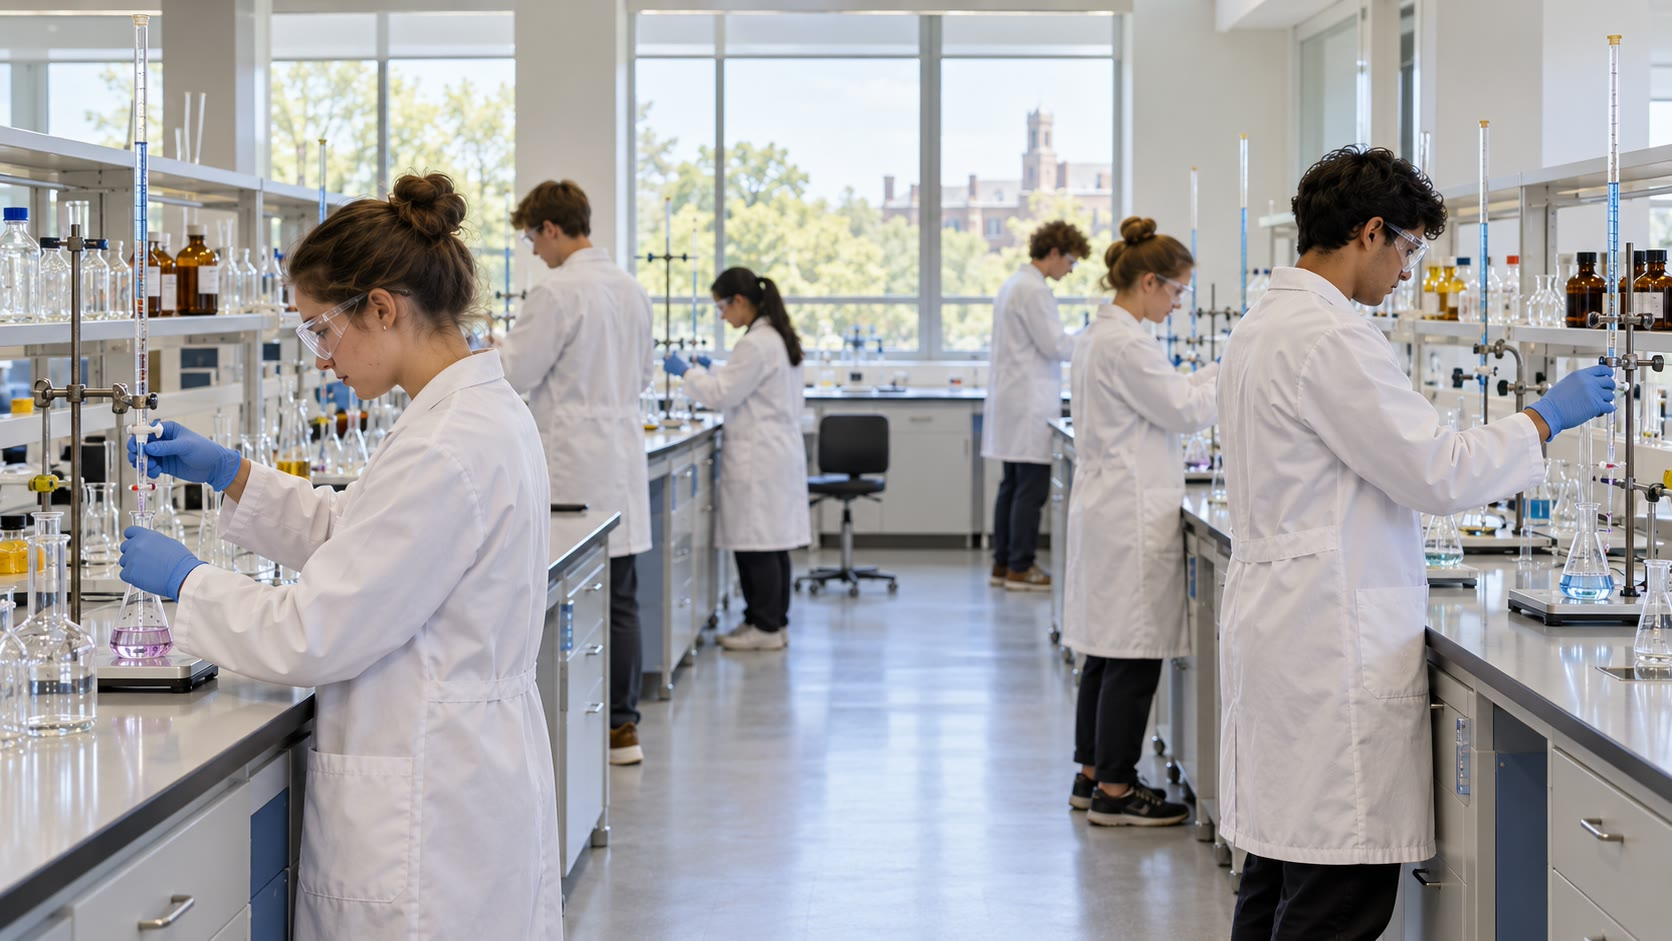
\includegraphics[width=0.66\linewidth]{images/book2/ai/b1-15-teaching-lab.jpg}

{\small Une salle de travaux pratiques~: une burette, un erlenmeyer sur
un agitateur magnétique, des gants et des lunettes. Le \omterm{def:b1:titration-methods:titration}{titrage} est la
mesure quantitative la plus courante en chimie.}
\end{omfigure}

\section{Titrage et équivalence}

\begin{definition}[Titrage, équivalence]\label{def:b1:titration-methods:titration}
Un \emph{titrage}\index{titrage} détermine la quantité de matière d'une
espèce, l'\emph{espèce titrée}\index{espece titree@espèce titrée}, par une réaction avec un réactif
de concentration connue, le \emph{réactif titrant}\index{reactif titrant@réactif titrant}, ajouté
progressivement. La réaction doit être unique, \omterm{def:b1:extent-q-and-k:quantitative}{quantitative} ($K$ grande)
et rapide. L'\emph{équivalence}\index{equivalence@équivalence} est atteinte lorsque le réactif
titrant et l'espèce titrée ont été mis en présence dans les proportions
stœchiométriques de la réaction~; le volume versé est alors le volume
équivalent, et le point de la courbe de titrage correspondant est le
\emph{point d'équivalence}\index{point d'equivalence@point d'équivalence}. Le volume auquel l'expérimentateur
s'arrête, en voyant un changement de couleur ou une rupture de pente,
est le \emph{point de fin de titrage}\index{point de fin de titrage}~; une bonne
méthode le fait coïncider avec l'équivalence.
\end{definition}

\begin{proposition}[Relation à l'équivalence]\label{prop:b1:titration-methods:equivalence}
Pour une réaction de \omterm{def:b1:titration-methods:titration}{titrage} $a\,\mathrm{A} + b\,\mathrm{B} \to \cdots$,
l'\omterm{def:b1:titration-methods:titration}{espèce titrée} A ($n_A$ mol) étant titrée par B à la concentration
$C_B$, le volume équivalent vérifie
\[
  \frac{n_A}{a} = \frac{C_B V_{\mathrm{eq}}}{b} .
\]
\end{proposition}

\begin{proof}
Soit $x$ l'\omterm{def:b1:extent-q-and-k:extent}{avancement} une fois versé un volume $V$ de \omterm{def:b1:titration-methods:titration}{réactif titrant}.
Avant l'\omterm{def:b1:titration-methods:titration}{équivalence}, B est limitant et, la réaction étant \omterm{def:b1:extent-q-and-k:quantitative}{quantitative},
$x = C_BV/b$~; après, A est limitant et $x = n_A/a$. L'\omterm{def:b1:titration-methods:titration}{équivalence} est le
volume pour lequel les deux sont épuisés ensemble, $n_A - ax = 0$ et
$C_BV - bx = 0$~: l'élimination de $x$ donne la relation.
\end{proof}

\section{Titrages directs et indirects}

\begin{definition}[Types de titrage]\label{def:b1:titration-methods:kinds}
Dans un \emph{titrage direct}\index{titrage direct}, le \omterm{def:b1:titration-methods:titration}{réactif titrant}
réagit avec l'\omterm{def:b1:titration-methods:titration}{espèce titrée} elle-même. Dans un \emph{titrage en
retour}\index{titrage en retour}, on ajoute à l'\omterm{def:b1:titration-methods:titration}{espèce titrée} un excès connu d'un réactif, et
l'on titre l'excès restant. Lorsqu'une solution contient plusieurs
espèces qui réagissent tour à tour avec le \omterm{def:b1:titration-methods:titration}{réactif titrant}, on les dose
par des \emph{titrages successifs}\index{titrages successifs}, une
\omterm{def:b1:titration-methods:titration}{équivalence} après l'autre~; lorsqu'elles réagissent ensemble et donnent
une seule \omterm{def:b1:titration-methods:titration}{équivalence}, par un \emph{titrage simultané}\index{titrage simultane@titrage simultané},
qui ne donne que leur somme.
\end{definition}

\begin{method}[Titrage en retour]\label{met:b1:titration-methods:back-titration}
On y recourt lorsque la réaction directe est lente, lorsque l'\omterm{def:b1:titration-methods:titration}{espèce
titrée} est instable ou volatile, ou lorsque aucun indicateur ne convient
à la réaction directe.
\begin{enumerate}
  \item Ajouter une quantité connue $n_R$ d'un réactif R, en excès, et le
        laisser réagir complètement avec l'\omterm{def:b1:titration-methods:titration}{espèce titrée} A
        ($\alpha\,\mathrm{A} + \rho\,\mathrm{R}$).
  \item Titrer l'excès de R par un \omterm{def:b1:titration-methods:titration}{réactif titrant} T ($\rho'\,\mathrm{R} +
        \tau\,\mathrm{T}$) jusqu'au volume équivalent $V_T$.
  \item Calculer $n_{R,\text{excès}} = \frac{\rho'}{\tau}C_TV_T$, puis
        $n_A = \frac{\alpha}{\rho}(n_R - n_{R,\text{excès}})$.
\end{enumerate}
\end{method}

Le problème du week-end titre ainsi la vitamine C~: l'acide ascorbique
réduit un excès de diiode, et le diiode restant est titré par le
thiosulfate.

\section{Titrages pH-métriques et indicateurs}

\begin{omfigure}
\begin{tikzpicture}[font=\small]
  \pic at (0,0) {stirrer};
  \pic at (0,0.18) {beaker={0.55}{omDef!14}};
  \pic at (0.2,2.45) {burette={0.75}{white}};
  \pic at (-0.45,0.45) {probe};
  \pic (m) at (-2.6,3.2) {meter={pH}};
  \draw[thick] (-0.45,3.45) to[out=90, in=0] (m-b);
  \node[anchor=west] at (0.65,6.2) {burette~: NaOH, \qty{0.100}{mol/L}};
  \node[anchor=west] at (1.0,1.0) {acide, $V_0 = \qty{10.0}{mL}$, dilué};
  \draw[<-, omProp, thick] (1.2,-0.25) -- (1.8,-0.25) node[anchor=west, text=black] {agitateur magnétique};
  \draw[<-, omProp, thick] (-0.62,2.4) -- (-1.5,2.0) node[anchor=east, text=black] {électrode combinée};
\end{tikzpicture}

{\small Un \omterm{def:b1:titration-methods:titration}{titrage} pH-métrique. L'électrode de verre combinée mesure le
pH après chaque ajout à la burette~; l'agitateur homogénéise la
solution. L'électrode est étalonnée au préalable avec deux \omterm{def:b1:predominant-reaction:buffer}{solutions
tampons}.}
\end{omfigure}

\begin{omfigure}
\begin{tikzpicture}
\begin{axis}[name=s,
  width=0.5\linewidth, height=5.6cm, xmin=0, xmax=20, ymin=0, ymax=14,
  axis x line=bottom, axis y line=left, xlabel={$V$ (mL)}, ylabel={pH},
  xtick={0,5,10,15,20}, ytick={0,2,4,6,8,10,12,14},
  tick label style={font=\small}, label style={font=\small}]
\addplot[omDef, very thick] table[x=V, y=pH] {figdata/out/bachelor-1-titration-curves-strong.dat};
\addplot[omProp, thick] table[x=V, y=pH] {figdata/out/bachelor-1-titration-curves-weak.dat};
\node[font=\scriptsize, omDef, anchor=south west] at (axis cs:6,0.2) {\ce{HCl}};
\node[font=\scriptsize, omProp, anchor=west] at (axis cs:0.4,6.4) {\ce{CH3COOH}};
\draw[dotted] (axis cs:5,0) -- (axis cs:5,4.76) -- (axis cs:0,4.76);
\node[font=\scriptsize, anchor=north] at (axis cs:2.5,4.7) {$\mathrm{p}K_a$};
\end{axis}
\begin{axis}[at={(s.east)}, anchor=west, xshift=1.2cm,
  width=0.5\linewidth, height=5.6cm, xmin=0, xmax=20, ymin=0, ymax=14,
  axis x line=bottom, axis y line=left, xlabel={$V$ (mL)}, ylabel={pH},
  xtick={0,5,10,15,20}, ytick={0,2,4,6,8,10,12,14},
  tick label style={font=\small}, label style={font=\small}]
\addplot[omMeth, very thick] table[x=V, y=pH] {figdata/out/bachelor-1-titration-curves-mixture.dat};
\node[font=\scriptsize, anchor=west, align=left] at (axis cs:10.8,6.0) {\ce{HCl} + \ce{CH3COOH}\\ deux équivalences};
\end{axis}
\end{tikzpicture}

{\small À gauche~: \qty{10.0}{mL} d'acide chlorhydrique et d'acide
éthanoïque, tous deux à \qty{0.100}{mol/L}, titrés par l'hydroxyde de
sodium à \qty{0.100}{mol/L}. L'\omterm{def:b1:predominant-reaction:strong-acid}{acide faible} présente une zone tampon où
le pH $=
\mathrm{p}K_a$ à la \omterm{def:b1:titration-methods:titration}{demi-équivalence}, et un \omterm{def:b1:titration-methods:titration}{point d'équivalence} à
pH 8.73. À droite~: un mélange à \qty{0.050}{mol/L} de chaque acide~:
l'\omterm{def:b1:predominant-reaction:strong-acid}{acide fort} est titré en premier (\omterm{def:b1:titration-methods:titration}{équivalence} à \qty{5}{mL}), puis
l'\omterm{def:b1:predominant-reaction:strong-acid}{acide faible} (\qty{10}{mL}).}
\end{omfigure}

\begin{proposition}[Demi-équivalence d'un acide faible]\label{prop:b1:titration-methods:half-equivalence}
Lorsqu'un \omterm{def:b1:predominant-reaction:strong-acid}{acide faible} HA est titré par une \omterm{def:b1:predominant-reaction:strong-acid}{base forte}, on a à la
\omterm{def:b1:titration-methods:titration}{demi-équivalence}
$\mathrm{pH} = \mathrm{p}K_a$, pourvu que l'acide ne soit ni trop fort
ni trop dilué ($\mathrm{p}K_a$ compris environ entre 4 et 10 à
\qty{0.1}{mol/L}).
\end{proposition}

\begin{proof}
À la \omterm{def:b1:titration-methods:titration}{demi-équivalence}, la \omterm{def:b1:extent-q-and-k:quantitative}{réaction quantitative} \ce{HA + OH- -> A- + H2O}
a transformé la moitié de HA~: $[\mathrm{HA}] = [\mathrm{A^-}]$, et la
relation de Henderson donne $\mathrm{pH} = \mathrm{p}K_a$. La condition
garantit que la réaction de HA avec l'eau et celle de $\mathrm{A^-}$ avec
l'eau ne modifient pas sensiblement ces quantités.
\end{proof}

\begin{proposition}[pH à l'équivalence d'un acide faible]\label{prop:b1:titration-methods:ph-at-equivalence}
À l'\omterm{def:b1:titration-methods:titration}{équivalence} du \omterm{def:b1:titration-methods:titration}{titrage} d'un \omterm{def:b1:predominant-reaction:strong-acid}{acide faible} ($\mathrm{p}K_a$) par une
\omterm{def:b1:predominant-reaction:strong-acid}{base forte}, la solution est celle de la base conjuguée à la
concentration $C'$ (après dilution), et
\[
  \mathrm{pH} = \tfrac12(\mathrm{p}K_e + \mathrm{p}K_a + \log C') .
\]
\end{proposition}

\begin{proof}
La \omterm{def:b1:predominant-reaction:predominant-reaction}{réaction prépondérante} de la base avec l'eau,
\ce{A- + H2O <=> HA + OH-}, a pour constante $K = K_e/K_a$~; la base
étant peu transformée, $[\ce{OH-}] = \sqrt{KC'}$
(\cref{prop:b1:predominant-reaction:ph-formulas}), d'où le résultat. Pour
l'acide éthanoïque, $C' = \qty{0.050}{mol/L}$~:
$\frac12(14.00 + 4.76 - 1.30) = 8.73$.
\end{proof}

\begin{proposition}[Titrages successifs]\label{prop:b1:titration-methods:successive}
Deux acides titrés par la même base donnent des \omterm{def:b1:titration-methods:titration}{équivalences} séparées,
chacune à mieux que \qty{1}{\percent} près, si leurs $\mathrm{p}K_a$
diffèrent d'au moins 4.
\end{proposition}

\begin{proof}
À la première \omterm{def:b1:titration-methods:titration}{équivalence}, la réaction de la base $\mathrm{A_1^-}$ avec
le second acide $\mathrm{HA_2}$, $\mathrm{A_1^-} + \mathrm{HA_2}
\rightleftharpoons \mathrm{HA_1} + \mathrm{A_2^-}$, a pour constante $K = 10^{\mathrm{p}K_1 - \mathrm{p}K_2}$.
À partir de quantités égales, la fraction $x$ du second acide déjà
titrée vérifie $x^2/(1 - x)^2 = K$~; pour $x \leqslant 0.01$, $K
\leqslant 10^{-4}$, c'est-à-dire $\mathrm{p}K_2 - \mathrm{p}K_1 \geqslant 4$.
\end{proof}

L'acide phosphorique (2.15, 7.21, 12.34) donne deux \omterm{def:b1:titration-methods:titration}{équivalences}
nettes~; la troisième se perd dans l'eau de la base. L'acide éthanoïque
mélangé à l'acide chlorhydrique (à droite sur la figure) est titré après
lui, l'\omterm{def:b1:predominant-reaction:strong-acid}{acide fort} se comportant comme un $\mathrm{p}K_a$ inférieur à 0.

\begin{method}[Repérer une équivalence sur une courbe]\label{met:b1:titration-methods:derivative}
\begin{enumerate}
  \item Dérivée~: calculer $\Delta\mathrm{pH}/\Delta V$ entre points
        successifs~; l'\omterm{def:b1:titration-methods:titration}{équivalence} correspond à son maximum.
  \item Tangentes~: tracer deux tangentes parallèles à la courbe de part
        et d'autre du saut, puis la parallèle équidistante~; elle coupe
        la courbe au \omterm{def:b1:titration-methods:titration}{point d'équivalence}.
\end{enumerate}
\end{method}

\begin{method}[Les tangentes, par le calcul]\label{met:b1:titration-methods:tangents}
Pour une courbe enregistrée par ordinateur, ajuster les points de chaque
côté du saut par une fonction régulière et prendre le point
d'inflexion~; pour un saut symétrique (\omterm{def:b1:predominant-reaction:strong-acid}{acide fort}, \omterm{def:b1:predominant-reaction:strong-acid}{base forte}), le
milieu du saut, à pH 7, est le \omterm{def:b1:titration-methods:titration}{point d'équivalence}.
\end{method}

\begin{definition}[Indicateur coloré, zone de virage]\label{def:b1:titration-methods:indicator}
Un \emph{indicateur coloré}\index{indicateur colore@indicateur coloré} est un \omterm{def:b1:predominant-reaction:bronsted}{couple acide/base} faible
HIn/In$^-$ dont les deux formes ont des couleurs différentes. Sa couleur
change sur la \emph{zone de virage}\index{zone de virage}, domaine de pH
où aucune des deux formes ne domine nettement, environ
$\mathrm{p}K_{a}(\mathrm{HIn}) \pm 1$.
\end{definition}

\begin{omfigure}
\begin{tabular}{lccl}
\hline
indicateur & $\mathrm{p}K_a$ & \omterm{def:b1:titration-methods:indicator}{zone de virage} & couleurs (acide / base) \\
\hline
hélianthine & 3.5 & 2.5--4.5 & rouge / jaune \\
rouge de méthyle & 4.8 & 3.8--5.8 & rouge / jaune \\
rouge de phénol & 7.9 & 6.9--8.9 & jaune / rouge \\
bleu de thymol (second virage) & 9.2 & 8.2--10.2 & jaune / bleu \\
\hline
\end{tabular}

\smallskip
{\small Quatre indicateurs, $\mathrm{p}K_a$ tirés d'une compilation
critique de \omterm{def:b1:complexation:formation-constant}{constantes de dissociation}~; les \omterm{def:b1:titration-methods:indicator}{zones de virage} valent
$\mathrm{p}K_a \pm 1$.}
% ledger: pka:methylorange, pka:methylred, pka:phenolred, pka:thymolblue2
\end{omfigure}

\begin{method}[Choisir un indicateur]\label{met:b1:titration-methods:choose-indicator}
Choisir un indicateur dont la \omterm{def:b1:titration-methods:indicator}{zone de virage} est incluse dans le saut
vertical de la courbe, aussi près que possible du pH à l'\omterm{def:b1:titration-methods:titration}{équivalence}.
\omterm{def:b1:predominant-reaction:strong-acid}{Acide fort} par \omterm{def:b1:predominant-reaction:strong-acid}{base forte} (saut de 3.3 à 10.7 pour $\pm\qty{0.1}{mL}$
ici)~: n'importe lequel des quatre. Acide éthanoïque (\omterm{def:b1:titration-methods:titration}{équivalence} à
8.73)~: rouge de phénol ou bleu de thymol~; l'hélianthine virerait bien
avant l'\omterm{def:b1:titration-methods:titration}{équivalence}.
\end{method}

\section{Titrages potentiométriques}

\begin{definition}[Titrage potentiométrique]\label{def:b1:titration-methods:potentiometric}
Un \emph{titrage potentiométrique}\index{titrage potentiometrique@titrage potentiométrique}
suit le potentiel d'une électrode plongée dans la solution par rapport à
une \omterm{def:b1:nernst:reference-electrode}{électrode de référence}, lors d'un \omterm{def:b1:titration-methods:titration}{titrage} d'oxydoréduction (fil de
platine), de précipitation (fil d'argent) ou de complexation.
\end{definition}

\begin{proposition}[Points remarquables d'un titrage d'oxydoréduction]\label{prop:b1:titration-methods:potentiometric-points}
Pour le \omterm{def:b1:titration-methods:titration}{titrage} de $\mathrm{Red_1}$ par $\mathrm{Ox_2}$ selon
$n_2\,\mathrm{Red_1} + n_1\,\mathrm{Ox_2} \to n_2\,\mathrm{Ox_1} +
n_1\,\mathrm{Red_2}$ (couples à $n_1$ et $n_2$ électrons), on a
$E(V_{\mathrm{eq}}/2) = E^\circ_1$, $E(2V_{\mathrm{eq}}) =
E^\circ_2$, et à l'\omterm{def:b1:titration-methods:titration}{équivalence}
\[
  E_{\mathrm{eq}} = \frac{n_1E^\circ_1 + n_2E^\circ_2}{n_1 + n_2},
\]
pour des couples dont les \omterm{def:b1:nernst:couple}{demi-équations} ne font intervenir aucune autre
espèce (ou à un pH qui maintient fixes les termes supplémentaires).
\end{proposition}

\begin{proof}
À la \omterm{def:b1:titration-methods:titration}{demi-équivalence}, la moitié de $\mathrm{Red_1}$ est oxydée~:
$[\mathrm{Ox_1}] = [\mathrm{Red_1}]$ et la \omterm{thm:b1:nernst:nernst}{relation de Nernst} du couple 1
donne $E^\circ_1$. À $2V_{\mathrm{eq}}$, il y a autant de
$\mathrm{Ox_2}$ en excès qu'il en a été réduit~:
$[\mathrm{Ox_2}] = [\mathrm{Red_2}]$, $E = E^\circ_2$. À l'\omterm{def:b1:titration-methods:titration}{équivalence},
on multiplie la \omterm{thm:b1:nernst:nernst}{relation de Nernst} du couple 1 par $n_1$, celle du
couple 2 par $n_2$, et on les additionne~; la stœchiométrie impose
$[\mathrm{Ox_1}]/[\mathrm{Red_1}] \cdot [\mathrm{Ox_2}]/[\mathrm{Red_2}] = 1$
(les quantités de $\mathrm{Red_1}$ et de $\mathrm{Ox_2}$ restantes sont
dans le même rapport que les produits), de sorte que les logarithmes
s'éliminent.
\end{proof}

Pour le fer(II) titré par le permanganate en milieu acide à
\qty{1}{mol/L}, $n_1 = 1$ et $n_2 =
5$~: $E_{\mathrm{eq}} = (0.77 + 5 \times 1.51)/6 = 1.39$~V. Le saut,
d'environ 0.8 à 1.5~V, est si grand que la fin du \omterm{def:b1:titration-methods:titration}{titrage} est nette~; en
pratique, le permanganate sert de son propre indicateur, sa couleur
violette persistant dès la première goutte en excès.

\begin{omfigure}
\begin{tikzpicture}
\begin{axis}[name=p,
  width=0.5\linewidth, height=5.6cm, xmin=0, xmax=20, ymin=0.6, ymax=1.6,
  axis x line=bottom, axis y line=left, xlabel={$V$ (mL)}, ylabel={$E$ (V)},
  xtick={0,5,10,15,20},
  tick label style={font=\small}, label style={font=\small}]
\addplot[omDef, very thick] table[x=V, y=E] {figdata/out/bachelor-1-titration-curves-potentiometric.dat};
\draw[dotted] (axis cs:5,0.6) -- (axis cs:5,0.77) -- (axis cs:0,0.77);
\draw[dotted] (axis cs:10,0.6) -- (axis cs:10,1.39) -- (axis cs:0,1.39);
\node[font=\scriptsize, anchor=south west] at (axis cs:0.2,0.77) {0.77};
\node[font=\scriptsize, anchor=south west] at (axis cs:0.2,1.39) {1.39};
\end{axis}
\begin{axis}[at={(p.east)}, anchor=west, xshift=1.2cm,
  width=0.5\linewidth, height=5.6cm, xmin=0, xmax=20, ymin=0, ymax=4.6,
  axis x line=bottom, axis y line=left, xlabel={$V$ (mL)},
  ylabel={$\kappa$ (mS/cm)}, xtick={0,5,10,15,20},
  tick label style={font=\small}, label style={font=\small}]
\addplot[omProp, very thick] table[x=V, y=kappa] {figdata/out/bachelor-1-titration-curves-conductimetric.dat};
\draw[dotted] (axis cs:10,0) -- (axis cs:10,1.15);
\end{axis}
\end{tikzpicture}

{\small À gauche~: \omterm{def:b1:titration-methods:potentiometric}{titrage potentiométrique} de \qty{10.0}{mL} de fer(II)
à \qty{0.100}{mol/L} par le permanganate à \qty{0.0200}{mol/L} en milieu
acide à \qty{1}{mol/L} (électrode de platine, potentiel par rapport à
l'électrode à hydrogène). À droite~: \omterm{def:b1:titration-methods:titration}{titrage} conductimétrique de
\qty{100}{mL} d'acide chlorhydrique à \qty{0.0100}{mol/L} par
l'hydroxyde de sodium à \qty{0.100}{mol/L}~; l'\omterm{def:b1:titration-methods:titration}{équivalence} se situe à
l'intersection de deux droites.}
% ledger: lam:H+, lam:OH-, lamsalt:HCl, lamsalt:NaCl (conductivities in figdata/bachelor-1/titration-curves.py)
\end{omfigure}

\section{Titrages conductimétriques, complexométriques et par précipitation}

\begin{definition}[Conductivité molaire ionique]\label{def:b1:titration-methods:conductivity}
La conductivité $\kappa$ d'une solution (en \unit{S/m}) mesure sa
capacité à transporter le courant par le mouvement de ses ions. La
\emph{conductivité molaire
ionique}\index{conductivite molaire ionique@conductivité molaire ionique} $\lambda_i$ d'un ion est sa contribution
par mole et par unité de volume~; sa valeur à dilution infinie,
$\lambda_i^\circ$, est une constante de l'ion et du solvant à une
température donnée.
\end{definition}

\begin{proposition}[Loi de Kohlrausch]\label{prop:b1:titration-methods:kohlrausch}
En solution diluée, la conductivité est la somme des contributions des
ions,
\[
  \kappa = \sum_i \lambda_i^\circ c_i ,
\]
c'est la \emph{loi de Kohlrausch}\index{loi de Kohlrausch}~; la
conductivité molaire d'un sel est la somme de celles de ses ions.
\end{proposition}

\admitted{La \omterm{prop:b1:titration-methods:kohlrausch}{loi de Kohlrausch} exprime que les ions dilués se déplacent
indépendamment~; ses limites aux concentrations plus élevées sont
étudiées dans le volume de deuxième année. On l'utilise ici comme une
loi expérimentale.}

\begin{proposition}[Pentes d'un titrage conductimétrique]\label{prop:b1:titration-methods:conductimetric-slopes}
Lorsqu'un \omterm{def:b1:predominant-reaction:strong-acid}{acide fort} H$^+$X$^-$ est titré par une \omterm{def:b1:predominant-reaction:strong-acid}{base forte}
Na$^+$OH$^-$ dans un grand volume (dilution négligée), la conductivité
varie linéairement avec le volume versé, avec une pente proportionnelle à
$\lambda^\circ(\ce{Na+}) - \lambda^\circ(\ce{H+}) < 0$ avant
l'\omterm{def:b1:titration-methods:titration}{équivalence} et à $\lambda^\circ(\ce{Na+}) + \lambda^\circ(\ce{OH-}) > 0$
après.
\end{proposition}

\begin{proof}
Avant l'\omterm{def:b1:titration-methods:titration}{équivalence}, chaque mole d'hydroxyde ajoutée retire une mole de
\ce{H+} (\ce{H+ + OH- -> H2O}) et apporte une mole de \ce{Na+}~; après
l'\omterm{def:b1:titration-methods:titration}{équivalence}, elle ajoute un \ce{Na+} et un \ce{OH-}. \ce{X-} reste
inchangé. D'après la \omterm{prop:b1:titration-methods:kohlrausch}{loi de Kohlrausch}, la conductivité varie de ces
combinaisons de $\lambda^\circ$ multipliées par la quantité ajoutée et
divisées par le volume (fixe).
\end{proof}

À partir des conductivités limites, $\lambda^\circ(\ce{H+}) =
\qty{349.8}{S.cm^2/mol}$ et $\lambda^\circ(\ce{OH-}) = 198.3$, et de
celles des sels \ce{HCl} (426) et \ce{NaCl} (126.5), la \omterm{prop:b1:titration-methods:kohlrausch}{loi de
Kohlrausch} donne
$\lambda^\circ(\ce{Cl-}) = 426 - 349.8 = 76.2$ et $\lambda^\circ(\ce{Na+}) =
126.5 - 76.2 = 50.3$~\unit{S.cm^2/mol}. Les ions hydrogène et hydroxyde
conduisent bien mieux que les autres~: la courbe est un V aigu.

Les \omterm{def:b1:titration-methods:titration}{titrages} complexométriques utilisent l'edta~: à pH 10 (tampon
ammoniacal), le calcium et le magnésium réagissent quantitativement avec
lui (constantes conditionnelles du \cref{ch:b1:complexation}), et un
indicateur, lui-même faible complexant du métal, change de couleur quand
l'edta lui prend les derniers ions métalliques --- c'est le \omterm{def:b1:titration-methods:titration}{titrage} de
la dureté de l'eau. Les \omterm{def:b1:titration-methods:titration}{titrages} par précipitation utilisent les ions
argent~: les chlorures sont titrés par le nitrate d'argent avec le
chromate comme indicateur (\cref{exo:b1:precipitation:8}), ou suivis à
l'aide d'une électrode d'argent (\cref{ch:b1:nernst}). La précision de
tous ces résultats, fixée par la verrerie et par le repérage de la fin
du \omterm{def:b1:titration-methods:titration}{titrage}, est traitée au \cref{ch:b1:lab-techniques-1}.

\section{Exercices}

\begin{exercise}[$\star$]\label{exo:b1:titration-methods:1}
\qty{20.0}{mL} d'une solution d'hydroxyde de sodium nécessitent
\qty{12.4}{mL} d'acide chlorhydrique à \qty{0.100}{mol/L}. Écrire la
réaction, sa constante, et calculer la concentration de la base.
\end{exercise}

\begin{exercise}[$\star$]\label{exo:b1:titration-methods:2}
Quel indicateur du tableau convient au \omterm{def:b1:titration-methods:titration}{titrage} de l'ammoniac
(\qty{0.10}{mol/L},
$\mathrm{p}K_a = 9.25$) par l'acide chlorhydrique à \qty{0.10}{mol/L}~?
Calculer d'abord le pH à l'\omterm{def:b1:titration-methods:titration}{équivalence}.
\end{exercise}

\begin{exercise}[$\star$]\label{exo:b1:titration-methods:3}
\qty{10.0}{mL} de fer(II) sont titrés par le permanganate à
\qty{0.0200}{mol/L}~; la couleur violette persiste à partir de
\qty{12.6}{mL}. Écrire la réaction et calculer la concentration du
fer(II).
\end{exercise}

\begin{exercise}[$\star$]\label{exo:b1:titration-methods:4}
Un échantillon d'eau de \qty{50.0}{mL} est titré par l'edta à
\qty{0.0100}{mol/L} à pH 10~; l'\omterm{def:b1:titration-methods:titration}{équivalence} est à \qty{14.2}{mL}.
L'edta réagit mole à mole avec le calcium et le magnésium. Calculer la
concentration totale de ces deux ions. S'agit-il d'un \omterm{def:b1:titration-methods:kinds}{titrage simultané}
ou de \omterm{def:b1:titration-methods:kinds}{titrages successifs}~?
\end{exercise}

\begin{exercise}[$\star\star$]\label{exo:b1:titration-methods:5}
Pour le \omterm{def:b1:titration-methods:titration}{titrage} de \qty{10.0}{mL} d'acide éthanoïque à \qty{0.100}{mol/L}
par l'hydroxyde de sodium à \qty{0.100}{mol/L}, calculer le pH à 0, 5.0,
10.0 et \qty{15.0}{mL} par les méthodes du
\cref{ch:b1:predominant-reaction}, et comparer à la courbe de ce
chapitre.
\end{exercise}

\begin{exercise}[$\star\star$]\label{exo:b1:titration-methods:6}
Montrer qu'un \omterm{def:b1:titration-methods:titration}{titrage} pH-métrique de l'acide phosphorique par
l'hydroxyde de sodium donne deux sauts, et calculer le pH à chaque
\omterm{def:b1:titration-methods:titration}{équivalence} pour un acide à \qty{0.100}{mol/L} (\qty{10.0}{mL}, base à
\qty{0.100}{mol/L}). Pourquoi n'y a-t-il pas de troisième saut~?
\end{exercise}

\begin{exercise}[$\star\star$]\label{exo:b1:titration-methods:7}
Un mélange d'acide chlorhydrique et d'acide éthanoïque (\qty{10.0}{mL})
est titré par l'hydroxyde de sodium à \qty{0.100}{mol/L}~: deux
\omterm{def:b1:titration-methods:titration}{équivalences}, à \qty{6.2}{mL} et à \qty{14.6}{mL}. Calculer les deux
concentrations. Quel est le pH à mi-chemin entre les deux
\omterm{def:b1:titration-methods:titration}{équivalences}~?
\end{exercise}

\begin{exercise}[$\star\star$]\label{exo:b1:titration-methods:8}
Calculer le potentiel de l'électrode de platine dans le \omterm{def:b1:titration-methods:titration}{titrage} du
fer(II) par le permanganate (données du chapitre) à 2.0, 9.0, 11.0 et
\qty{20.0}{mL}.
\end{exercise}

\begin{exercise}[$\star\star$]\label{exo:b1:titration-methods:9}
À l'aide de la \omterm{prop:b1:titration-methods:kohlrausch}{loi de Kohlrausch} et des valeurs du chapitre, calculer la
conductivité de l'acide chlorhydrique titré à 0, 10.0 et
\qty{20.0}{mL} de base (\qty{100}{mL} d'acide à \qty{0.0100}{mol/L},
base à \qty{0.100}{mol/L}, dilution prise en compte), ainsi que les deux
pentes.
\end{exercise}

\begin{exercise}[$\star\star\star$]\label{exo:b1:titration-methods:10}
Démontrer que la courbe pH-métrique d'un \omterm{def:b1:predominant-reaction:strong-acid}{acide fort} titré par une \omterm{def:b1:predominant-reaction:strong-acid}{base
forte} est symétrique par rapport au \omterm{def:b1:titration-methods:titration}{point d'équivalence} lorsqu'on
néglige la dilution, et calculer l'amplitude du saut entre
$V_{\mathrm{eq}} \pm 0.1$~mL
pour le \omterm{def:b1:titration-methods:titration}{titrage} du chapitre. Comment change-t-elle si toutes les
concentrations sont divisées par 100~?
\end{exercise}

\begin{exercise}[$\star\star\star$]\label{exo:b1:titration-methods:11}
Établir l'équation de la courbe potentiométrique du fer(II) titré par le
permanganate avant et après l'\omterm{def:b1:titration-methods:titration}{équivalence}, et vérifier les trois points
remarquables de la \cref{prop:b1:titration-methods:potentiometric-points}.
Comment le potentiel à l'\omterm{def:b1:titration-methods:titration}{équivalence} changerait-il à pH 1~?
\end{exercise}

\begin{exercise}[$\star\star\star$]\label{exo:b1:titration-methods:12}
Le chlorure d'ammonium (\qty{0.100}{mol/L}, $\mathrm{p}K_a = 9.25$) ne
peut pas être titré avec précision par l'hydroxyde de sodium à l'aide
d'un indicateur. L'expliquer à partir de la courbe, puis proposer un
\omterm{def:b1:titration-methods:kinds}{titrage en retour}~: excès d'hydroxyde de sodium, élimination de
l'ammoniac par ébullition, \omterm{def:b1:titration-methods:titration}{titrage} de l'hydroxyde restant par l'acide
chlorhydrique. Écrire le calcul.
\end{exercise}

\section{Problème~: combien de vitamine C dans le comprimé~?}

\begin{problem}[{Problème du week-end --- la réaction du diiode sur
l'acide ascorbique, un titrage en retour par le thiosulfate, le calcul
du résultat et de son incertitude, pour aboutir à la masse d'acide
ascorbique par comprimé}]
\label{pb:b1:titration-methods:1}
Un comprimé est broyé et dissous dans l'eau dans une fiole jaugée de
\qty{100.0}{mL}. On prélève à la pipette une partie aliquote de
\qty{10.00}{mL}, à laquelle on ajoute \qty{20.00}{mL} de solution de
diiode à \qty{0.0250}{mol/L} (excès). Le diiode restant est titré par
le thiosulfate de sodium à \qty{0.0500}{mol/L}, avec l'empois d'amidon
comme indicateur~: la couleur bleue disparaît à \qty{8.90}{mL}. L'acide
ascorbique a pour formule \ce{C6H8O6} ($M = \qty{176.0}{g/mol}$)~; le
diiode l'oxyde en \ce{C6H6O6}. $E^\circ(\ce{I2}/\ce{I-}) = 0.53$~V,
$E^\circ(\ce{S4O6^2-}/\ce{S2O3^2-}) = 0.02$~V.

\medskip
\noindent\textbf{Partie I --- Les réactions.}
\begin{enumerate}
  \item Écrire la \omterm{def:b1:nernst:couple}{demi-équation} du couple \ce{C6H6O6}/\ce{C6H8O6}.
  \item Écrire la réaction du diiode sur l'acide ascorbique.
  \item Donner le \omterm{def:b1:nernst:oxidation-number}{nombre d'oxydation} de l'iode dans \ce{I2} et \ce{I-}.
  \item Écrire la réaction du diiode avec le thiosulfate et calculer sa
        constante.
  \item L'empois d'amidon donne avec le diiode une couleur bleu foncé.
        Pourquoi la couleur disparaît-elle exactement à l'\omterm{def:b1:titration-methods:titration}{équivalence} du
        \omterm{def:b1:titration-methods:titration}{titrage} par le thiosulfate~?
  \item L'acide ascorbique est lentement oxydé par le dioxygène de
        l'air. En quoi cela plaide-t-il pour un ajout immédiat du diiode,
        en excès~?
\end{enumerate}

\medskip
\noindent\textbf{Partie II --- Pourquoi un \omterm{def:b1:titration-methods:kinds}{titrage en retour}~?}
\begin{enumerate}[resume]
  \item Que demanderait un \omterm{def:b1:titration-methods:kinds}{titrage direct} de l'acide ascorbique par le
        diiode~?
  \item Décrire le \omterm{def:b1:titration-methods:kinds}{titrage en retour} selon les trois étapes de la
        \cref{met:b1:titration-methods:back-titration}.
  \item Pourquoi le diiode doit-il être en excès~? Le vérifier sur le
        résultat.
  \item Pourquoi étalonne-t-on la solution de thiosulfate peu avant
        l'emploi~?
  \item La partie aliquote est de \qty{10.00}{mL} sur \qty{100.0}{mL}~:
        quel est le facteur de dilution~?
  \item Quelle verrerie délivre les \qty{20.00}{mL} de solution de
        diiode~?
\end{enumerate}

\medskip
\noindent\textbf{Partie III --- Le calcul.}
\begin{enumerate}[resume]
  \item Calculer la quantité de diiode introduite.
  \item Calculer la quantité de thiosulfate utilisée.
  \item En déduire la quantité de diiode en excès.
  \item En déduire la quantité de diiode qui a réagi avec l'acide
        ascorbique.
  \item Calculer la quantité d'acide ascorbique dans la partie aliquote.
  \item Calculer la quantité, puis la masse, d'acide ascorbique dans le
        comprimé.
  \item Comparer à l'étiquette (\qty{500}{mg}).
\end{enumerate}

\medskip
\noindent\textbf{Partie IV --- Quelle confiance~?}
Les tolérances sont~: fiole \qty{100.0 \pm 0.1}{mL}, pipettes
\qty{10.00 \pm 0.02}{mL} et \qty{20.00 \pm 0.03}{mL}, lecture de la
burette $\pm\qty{0.05}{mL}$~; les deux concentrations sont connues à
\qty{0.2}{\percent} près.
\begin{enumerate}[resume]
  \item Exprimer $n(\text{acide ascorbique})$ dans le comprimé en
        fonction des grandeurs mesurées.
  \item Quelles incertitudes relatives interviennent dans la quantité de
        diiode introduite et dans la quantité en excès~?
  \item Pourquoi une différence de deux quantités amplifie-t-elle
        l'incertitude relative~?
  \item En combinant les contributions comme au
        \cref{ch:b1:lab-techniques-1} (somme quadratique), estimer
        l'incertitude relative du résultat.
  \item Donner la masse d'acide ascorbique par comprimé avec son
        incertitude, à deux chiffres significatifs.
\end{enumerate}
\end{problem}
